\documentclass[9pt]{exam}
\usepackage[utf8]{inputenc}
\usepackage{amsmath,amsthm,amsfonts,amssymb,amscd}
\usepackage{multirow,booktabs}
\usepackage{enumitem}
\usepackage{fancyhdr}
\usepackage{mathrsfs}
\usepackage{wrapfig}
\usepackage{setspace}
\usepackage{calc}
\usepackage{subfig}
\usepackage{multicol}
\usepackage{cancel}
\usepackage[retainorgcmds]{IEEEtrantools}
\usepackage{framed}
\usepackage[most]{tcolorbox}
\usepackage{tikz}
\usepackage{geometry}
\geometry{
	a4paper,
	total={170mm,257mm},
	left=20mm,
	top=20mm,
}
\title{Electrostatics}
\author{Aaron G.K.}

\begin{document}
	\maketitle
	\begin{center}
		\section*{Charges \& Fields}	
	\end{center}
	Electromagnetism is a broad field of physics which studies about electromagnetic interaction and it also happens to be one of the four fundamental forces in nature. A subfield is electrostatics which is the study of charges at rest. Electrostatics is manifested in various walks of life and has been studied throughout scientific history. \\ \\ For example, the Italian scientist Luigi Galvani (1737–1798) performed a series of experiments in which static electricity was used to stimulate contractions of leg muscles of dead frogs, an effect already known in humans subjected to static discharges. But Galvani also found that if he joined two metal wires (say copper and zinc) end to end and touched the other ends to muscles, he produced the same effect in frogs as static discharge. \\ \\ Alessandro Volta (1745–1827), partly inspired by Galvani’s work, experimented with various combinations of metals and developed the battery. During the same era, other scientists made progress in discovering fundamental connections. The periodic table was developed as the systematic properties of the elements were discovered. This influenced the development and refinement of the concept of atoms as the basis of matter. Such submicroscopic descriptions of matter also help explain a great deal more. Atomic and molecular interactions, such as the forces of friction, cohesion, and adhesion, are now known to be manifestations of the electromagnetic force. \\ \\ Static electricity is just one aspect of the electromagnetic force, which also includes moving electricity and magnetism. 	All the macroscopic forces that we experience directly, such as the sensations of touch and the tension in a rope, are due to the electromagnetic force, one of the four fundamental forces in nature. The gravitational force, another fundamental force, is actually sensed through the electromagnetic interaction of molecules, such as between those in our feet. (The other two fundamental forces, the strong nuclear force and the weak nuclear force, cannot be sensed on the human scale.)\\
	\subsection*{Static Electricity}
	Many of the characteristics of static electricity can be explored by rubbing things together. Static cling generated in the attraction of straw to recently polished amber also result from rubbing. Similarly, lightning results from air movements under certain weather conditions. You can also rub a balloon on your hair, and the static electricity created can then make the balloon cling to a wall. \\ \\
	\textbf{Characteristics of static electricity include}:
	\begin{itemize}
		\item The effects of static electricity are explained by a physical quantity not previously introduced, called electric charge.
		\item There are only two types of charge, one called positive and the other called negative.
		\item Like charges repel, whereas unlike charges attract.
		\item The force between charges decreases with distance.
	\end{itemize}
	Charges are usually carried by subatomic particles like protons and electrons. The charges of electrons and protons are identical in magnitude but opposite in sign. Furthermore, all charged objects in nature are integer-multiples of this basic quantity of charge, meaning that all charges are made of combinations of a basic unit of charge(elementary charge). Usually, charges are formed by combinations of electrons and protons. The magnitude of this elementary charge is
	$$\text{q}_\text{e}=1.60\times10^{-19}\text{C}$$ The symbol \textbf{q} is commonly used for charge and the subscript \textbf{e} indicates the charge of a single electron (or proton).
	The SI unit of charge is the coulomb (C). Since any charge in the universe is an integral multiple of the elementary charge, we have the following:
	$$\text{Q}=\text{nq}_\text{e}$$
	\subsection*{Law of Conservation of Charge}
	The total charge is constant in any process. \begin{center}
		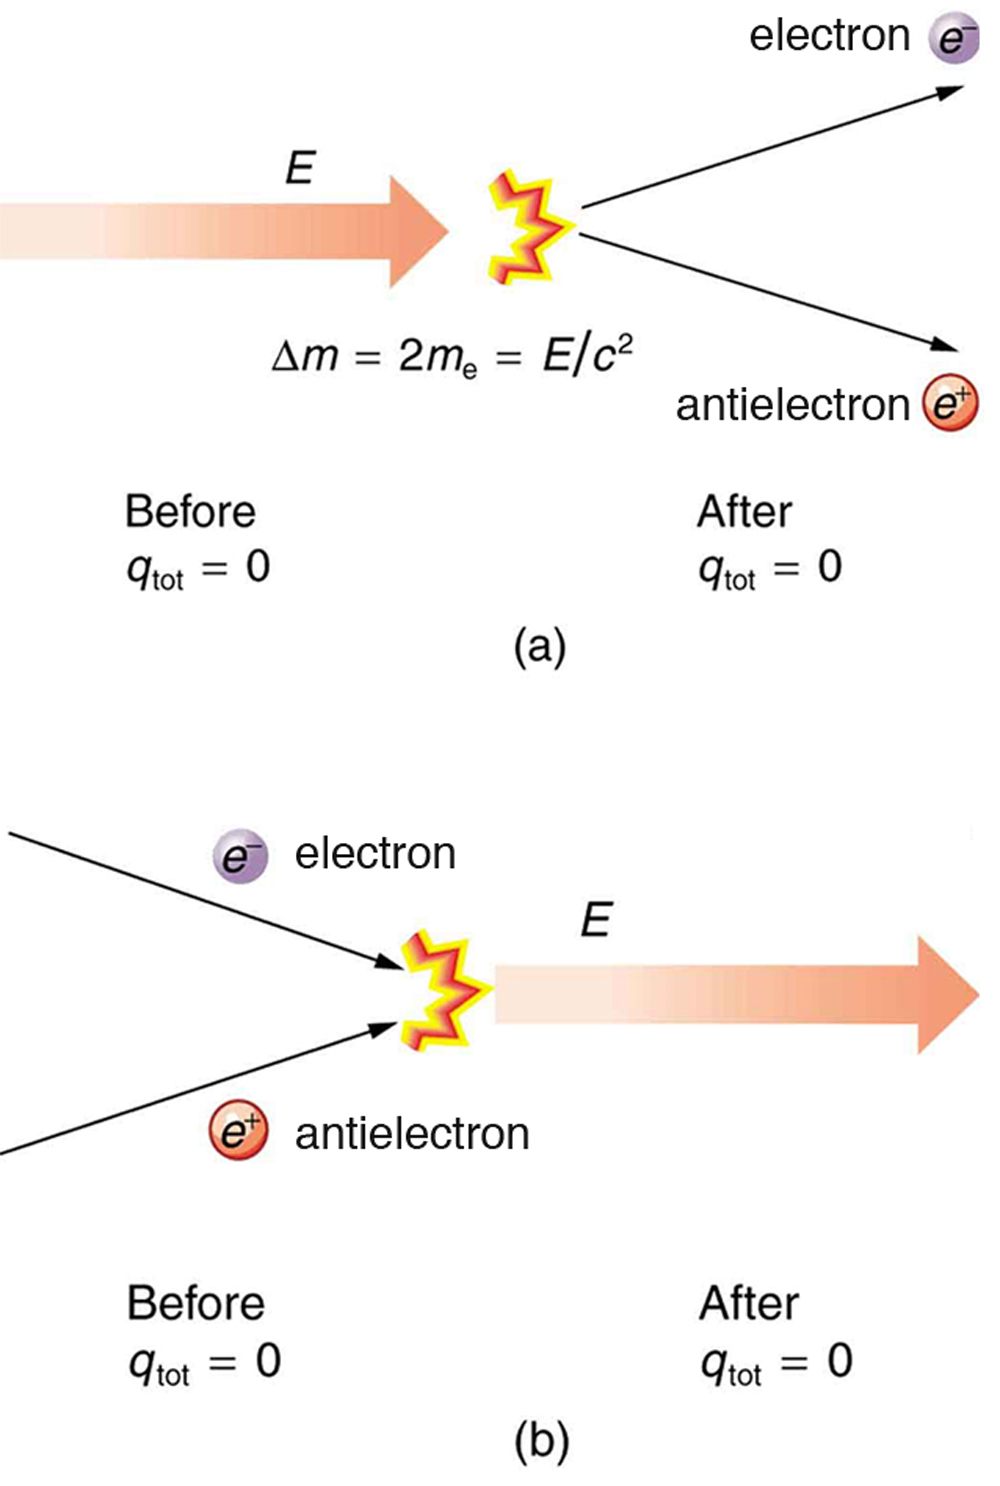
\includegraphics[scale=0.3]{charge_conservation.jpg}
	\end{center}
	In particle accelerators, mass can be created from energy. Sometimes, the created mass is charged, such as when an electron is created. Whenever a charged particle is created, another having an opposite charge is always created along with it, so that the total charge created is zero(because the net charge of a system is conserved). Usually, the two particles are “matter-antimatter” counterparts. For example, in the figure above: an antielectron would usually be created at the same time as an electron. The antielectron has a positive charge (it is called a positron), and so the total charge created is zero. Similarly, when an electron and a positron come together, they destroy each other and energy is formed from them.
	\subsection*{Charge Transfer} 
	Since charge is conserved, we can't create nor destroy it. However, we can transfer charges by various methods. Before we discuss those, let's review conductors \& insulators.  Some electrons in metals are not bound to individual atoms or sites in the material. These free electrons can move very freely. Any substance that has free electrons and allows charge to move relatively freely through it is called a conductor, materials that don't allow electrons to flow through them easily are called insulators. Here are some ways we can transfer charges:
	\subsubsection*{Conduction}
	An electroscope is being charged by touching it with a positively charged glass rod in the figure below.
	\begin{center}
		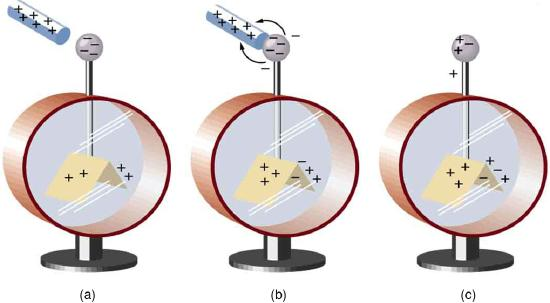
\includegraphics[scale=0.3]{electroscope}
	\end{center} Because the glass rod is an insulator, it must actually touch the electroscope to transfer charge to or from it. Since only electrons move in metals, we see that they are attracted to the top of the electroscope. There, some are transferred to the positive rod by touch, leaving the electroscope with a net positive charge. Electrostatic repulsion in the leaves of the charged electroscope separates them. The electrostatic force has a horizontal component that results in the leaves moving apart. Similarly, the electroscope can be negatively charged by contact with a negatively charged object.
	\subsubsection*{Induction}	 
	Induction is best done with the induced polarization of neutral objects. Polarization is the separation of charges in an object that remains neutral. Look at the figure below for instance.
	\begin{center}
		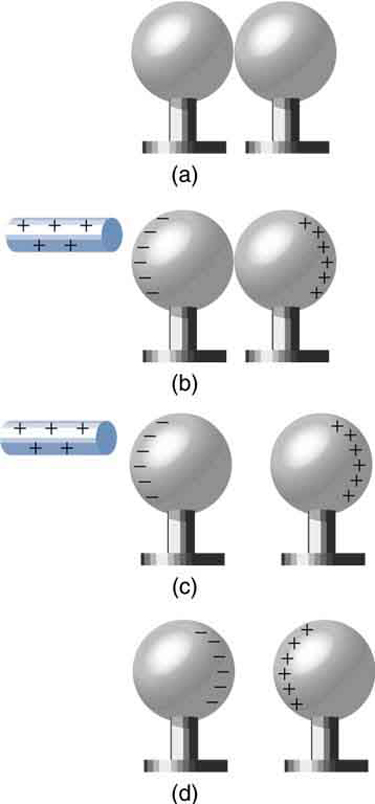
\includegraphics[scale=0.4]{induction}
	\end{center}If the spheres are now separated (before the rod is pulled away), each sphere will have a net charge. Note that the object closest to the charged rod receives an opposite charge when charged by induction. \\ \\
	Neutral objects(if they can be polarized) can be attracted to any charged object. The pieces of straw attracted to polished amber are neutral, for example. If you run a plastic comb through your hair, the charged comb can pick up neutral pieces of paper
	\subsection*{Cuolomb's Law}
	The mathematical formula for the electrostatic force is called Coulomb’s law after the French physicist Charles de Coulomb, who performed experiments and first proposed a formula to calculate it.
	\begin{quotation}
		Coulomb’s law calculates the magnitude of the force  F  between two point charges,  $\text{q}_1\text{  and  q}_2$ , separated by a distance r:
		$$\text{F}=\dfrac{\text{kq}_1\text{q}_2}{\text{r}^2}$$
		Where k is a constant which has a value of $\text{k}=\dfrac{1}{4\pi\epsilon_0}=8.99\times10^{9}\text{Nm}^2/\text{C}^2$
	\end{quotation}
	\subsection*{Electric Field}
	We have seen various types of forces so far. Most forces we experience daily are forces manifested through contact, but forces like the Cuolomb Force and gravity happen at a distance and don't necessarily need contact to be experienced or felt. Such forces are exerted through force fields. A field is generally a region in space such that a force is experienced. It is a way of conceptualizing and mapping the force that surrounds any object and acts on another object at a distance without apparent physical connection. For example, a charged rubber comb attracts neutral bits of paper from a distance by the Coulomb force. It is very useful to think of an object being surrounded in space by a force field. The force field carries the force to another object (called a test object) some distance away.  \\ \\
	Similarly, the Coulomb force field surrounding any charge extends throughout space. Using Coulomb’s law,  $\text{F}=\dfrac{\text{kq}_1\text{q}_2}{\text{r}^2}$, its magnitude is given by the equation  $\text{F}=\dfrac{\text{kQq}}{\text{r}^2}$ , for a point charge (a particle having a charge Q) acting on a test charge  q at a distance r. Both the magnitude and direction of the Coulomb force field depend on  Q  and the test charge  q . \\ \\
	To simplify things, we would prefer to have a field that depends only on the source Q and not on the test charge q. The electric field is defined in such a manner that it represents only the charge creating it and is unique at every point in space. Specifically, the electric field E is defined to be the ratio of the Coulomb force to the test charge:
	$$\mathbf{E}=\dfrac{\mathbf{F}}{\text{q}},$$ where  \textbf{F}  is the electrostatic force exerted on a positive test charge q.  It is important to note that  \textbf{E}  and \textbf{F} act in the same direction. It is also assumed that q is so small that it does not alter the charge distribution created by the source charge Q. According to Coulomb’s law, the force Q exerts on a test charge q is $\text{F}=\dfrac{\text{kQq}}{\text{r}^2}$. Thus the magnitude of the electric field, E , for a point charge is: 
	$$E=|\dfrac{F}{q}|=k|\dfrac{qQ}{qr^{2}}|=k\dfrac{|Q|}{r^{2}}.$$
	$$E=k\dfrac{|Q|}{r^{2}}$$
	Thus, we can see that the electric field by the source charge is to depend only on the charge Q and the distance r.
	\subsubsection*{Representing Field}
	To represent electric fields or fields in general, we use electric field lines. The lines are useful in visualizing field strength and direction. The electric field lines are defined for positive test charges(conventionally), and thus they show the direction of the force by a source charge acting on a positive charge. With that in mind, if we construct field lines for positive \& negative source charges, we get the following: \\ \\
	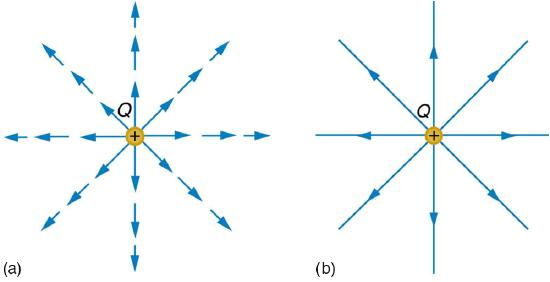
\includegraphics[scale=0.3]{source_p}\hspace{1in}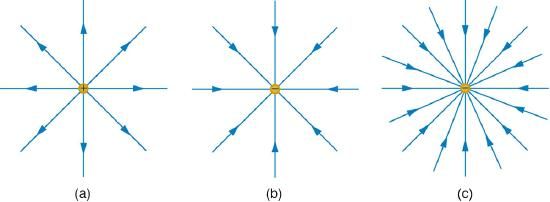
\includegraphics[scale=0.4]{source_n} \\
	On the left we have a positive source charge with an electric field around it while we have a negative source charge on the right. Although field lines are great tools, they are hypothetical. The properties of electric field lines for any charge distribution can be summarized as follows: \begin{itemize}
		\item Field lines must begin on positive charges and terminate on negative charges, or at infinity in the hypothetical case of isolated charges.
		\item The number of field lines leaving a positive charge or entering a negative charge is proportional to the magnitude of the charge.
		\item The strength of the field is proportional to the closeness of the field lines—more precisely, it is proportional to the number of lines per unit area perpendicular to the lines.
		\item The direction of the electric field is tangent to the field line at any point in space.
		\item Field lines can never cross.
	\end{itemize}
		\begin{center}
		\section*{Electric Potential and Potential Energy}	
	\end{center}
	When a free positive charge  q  is accelerated by an electric field, it is given kinetic energy. The process is analogous to an object being accelerated by a gravitational field. It is as if the charge is going down an electrical hill where its electric potential energy is converted to kinetic energy. 
	\begin{center}
		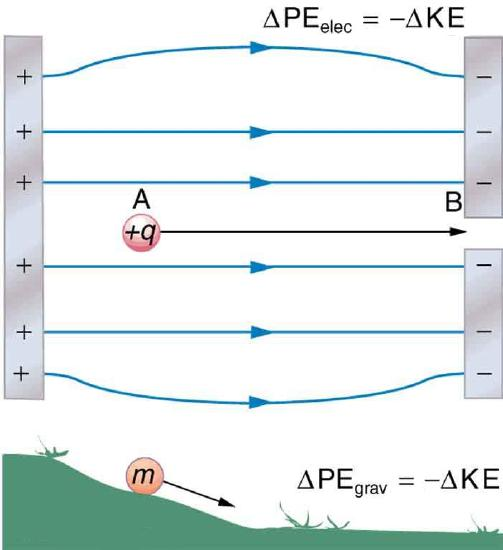
\includegraphics[scale=0.5]{pe_analogy}
	\end{center}
	The electrostatic force is conservative, which means that the work done on q is independent of the path taken(it also conserves the mechanical energy). This is exactly analogous to the gravitational force in the absence of dissipative forces such as friction. When a force is conservative, it is possible to define a potential energy associated with the force, and it is usually easier to deal with the potential energy (because it depends only on position) than to calculate the work directly. \\ \\
	We use the letters PE to denote electric potential energy, which has units of joules (J). The change in potential energy, $\varDelta$PE, is crucial, since the work done by a conservative force is the negative of the change in potential energy; that is, W=$-\varDelta$PE. For example, work W done to accelerate a positive charge from rest is positive and results from a loss in PE, or a negative $\varDelta$PE. There must be a minus sign in front of $\varDelta$PE to make W positive. PE can be found at any point by taking one point as a reference and calculating the work needed to move a charge to the other point. \\ \\
	We can show that the potential energy is equal to the work done as follows. We know that the mechanical energy is conserved in the presence of conservative forces. 
	$$\text{ME}_i=\text{ME}_f$$
	$$\text{KE}_i+\text{PE}_i=\text{KE}_f+\text{PE}_f$$
	We can rearrange the above equation as follows:
	$$\text{KE}_i-\text{KE}_f=\text{PE}_f-\text{PE}_i$$
	$$-\Delta\text{KE}=\Delta\text{PE}$$
	According to the work-kinetic energy theorem, the change in kinetic energy is the work done. As such, we have the following:
	$$-\Delta\text{W}=\Delta\text{PE}$$
	$$\Delta\text{PE}=-\Delta\text{W}$$
	W=$-\Delta$PE . For example, work  W  done to accelerate a positive charge from rest is positive and results from a loss in PE, or a negative  $\Delta$PE  there must be a negative sign in front of  $\Delta$ PE  to make  W  positive. PE can be found at any point by taking one point as a reference and calculating the work needed to move a charge to the other point.\\ \\
	We know that the potential energy is the work done by the conservative forces. Calculating the work directly is generally difficult, since  the direction and magnitude of F can be complex for multiple charges, for odd-shaped objects, and along arbitrary paths. But we do know that, since  F=qE , the work, and hence  $\Delta$PE , is proportional to the test charge  q. To have a physical quantity that is independent of test charge, we define electric potential  V to be the potential energy per unit charge:
	$$V=\dfrac{\text{PE}}{q}$$
	Since PE is proportional to  q, the dependence on  q  cancels. Thus  V  does not depend on  q. The change in potential energy  $\Delta$PE  is crucial, and so we are concerned with the difference in potential $\Delta$V  between two points, called the \textit{potential difference} or \textit{voltage}. \\ \\
	Thus, for two arbitrary points A \& B near a source charge, the potential difference is given by:
	$$\Delta V =V_{B}-V_{A}=\dfrac{\Delta \text{PE}}{q}.$$ 
	The SI unit of V is Volt, after Alessandro Volta. It is important to note that $1 \text{V}=1\dfrac{\text{J}}{\text{C}}$ \\ 
	\subsubsection*{Important note on voltage}
	The term \textbf{voltage} is the common name for potential difference. Keep in mind that whenever we say voltage , it is understood to be the potential difference between two points. For example, every battery has two terminals, and its voltage is the potential difference between them. \textit{\textbf{More fundamentally, the point you choose to be zero volts is arbitrary}}. This is analogous to the fact that gravitational potential energy has an arbitrary zero, such as the ground from which we measure the height from. \\ \\
	It is also imperative to note that voltage is not the same as energy. Voltage is the energy per unit charge. Thus a remote control battery and a flashlight battery can both have the same voltage (the same potential difference between battery terminals), yet one stores much more energy than the other since $\Delta$PE=q$\Delta$V. The car battery can move more charge than the motorcycle battery, although could be 1.5 V batteries.
	\subsubsection*{Relationship with Electric Field}
	For a simple and uniform electric field, we can relate the electric field to the potential. For example, a uniform electric field E is produced by placing a potential difference $\Delta$V across two parallel metal plates as shown below.
	\begin{center}
		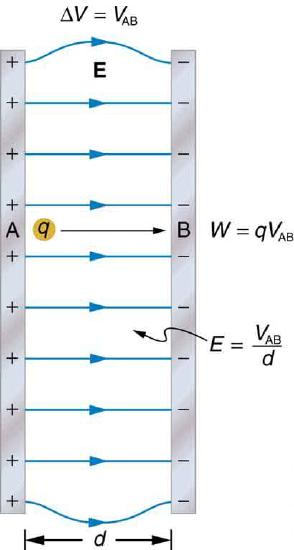
\includegraphics[scale=0.3]{metal_plates_v}
	\end{center}
	The work done to move the charge from the higher potential to the lower potential is:
	$$\text{W}=-\Delta \text{PE}=-q\Delta V=qV_{\text{AB}}\text{, where V}_{\text{AB}}\text{ is the potential difference between A and B}$$
	We know that the work done is given by W=Fd. Since F=qE, we see that W=qEd. Thus,
	$$\text{q}V_{\text{AB}}=\text{qEd}\text{, therefore,}$$
	$$V_{\text{AB}}=\text{Ed}$$
	Thus, for a uniform electric field, we can relate the electric field strength to the potential difference as shown above.
	\subsubsection*{Equipotential Lines \& Surfaces}
	We have seen above that potential is defined as the potential energy per unit charge. Thus, for a point source charge Q, the absolute potential at a distance r is given as follows:
	$$\text{V}=\dfrac{\text{PE}}{\text{q}}$$
	We know that the potential energy between the source charge Q and the test charge q is given by:
	$$\text{PE}=\dfrac{\text{KQq}}{\text{r}}$$
	Substituting this to the equation above, we get:
	$$\text{V}=\dfrac{\dfrac{\text{KQq}}{\text{r}}}{\text{q}}$$
	$$\text{V}=\dfrac{\text{KQ}}{\text{r}}$$
	Thus, a point charge's potential only depends on its magnitude and the distance from itself. For a positive point charge Q, we have its electric field as follows and as we are equidistant from the charge, we can infer that the potential is the same. The circle we see in the figure below is called an equipotential surface.\begin{center}
		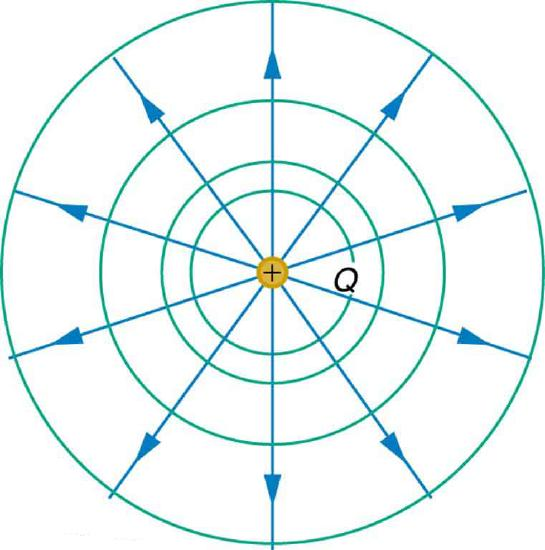
\includegraphics[scale=0.2]{equip_1}
	\end{center}
	However, as the number of charges changes, the geometry of equidistant surfaces also changes. For two charges, for example, here is the equipotential surface. We can see that it is far from being a circle. \begin{center}
		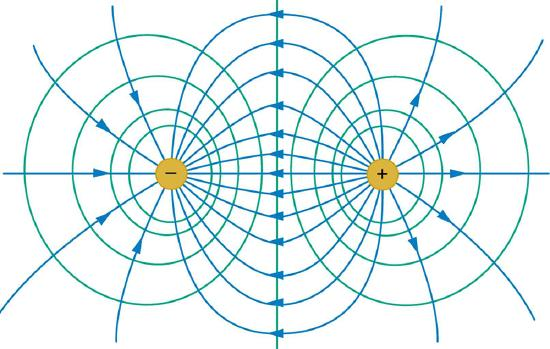
\includegraphics[scale=0.27]{equip_2}
	\end{center}
	You can also note that the equipotential surfaces are perpendicular to the electric field lines. \\ \\
	\subsubsection*{Grounding}
	A conductor is an equipotential surface in static situations. There can be no voltage difference across the surface of a conductor, or else it means that charges will flow. One of the uses of this fact is that a conductor can be fixed at zero volts by connecting it to the earth with a good conductor — a process called \textbf{grounding}. Grounding can be a useful safety tool. For example, grounding the metal case of an electrical appliance ensures that it is at zero volts relative to the earth.
		\subsection*{Capacitors}
	A capacitor is an electrical equipment that we use to store charge. We also use other electrical devices such as a battery to store charges, but the difference is that a capacitor stores more charge at a lower potential. The simplest form of a capacitor contains two metal plates separated by a small distance we an insulator between them. Below, you will find a schematic diagram of a simple capacitor.
	
	\begin{figure}[htp]
		\centering
		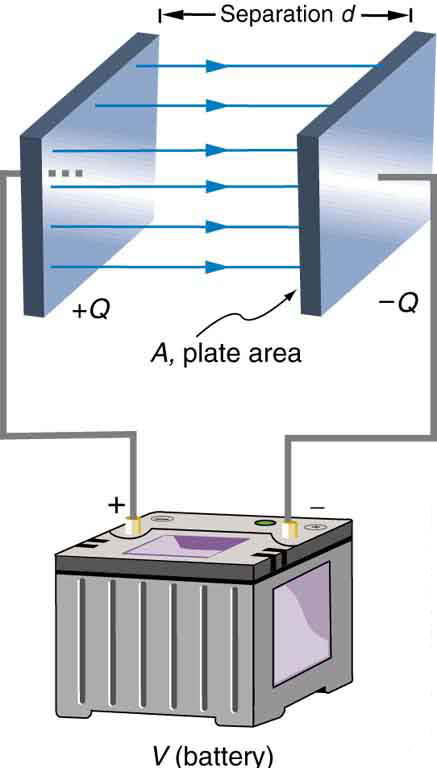
\includegraphics[width=4cm]{structure}
		\caption{The structure of a simple capacitor}
		\label{fig:structure}
	\end{figure}
	
	\subsection*{Concepts involving capacitors}
	\textbf{Capacitance} \newline
	Is the charge needed for each volt rise in the potential. In other words, it is how much charge can be stored within a given potential difference. That is,
	$$	C = \frac{Q}{V} $$
	Where:
	\begin{equation*}
		\begin{split}
			C = \text{Capacitance} \\
			Q = \text{Charge stored} \\
			V = \text{Potential difference/voltage between the plates}\\
		\end{split}
	\end{equation*}
	The SI unit of capacitance is called the Farad(in honor of Michael Faraday)
	, where 
	\begin{equation}
		1 F = \frac{1C}{1V}
	\end{equation}
	As we said earlier, capacitors are elements of circuits. Thus, we need special representation(symbols) for them so that we can know where they are located in circuits. In the diagram below, we see the representation of a capacitor in a circuit. Based on the type of capacitor it is, it might have different representations, but the first one will do for most of the topics we will be covering. 
	\begin{center}
		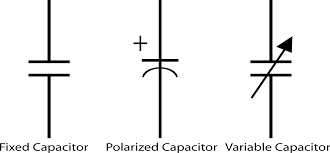
\includegraphics[scale=0.7]{cap.png}
		\label{fig:cap}
	\end{center}
	To understand how capacitors work, let's consider parallel plate capacitors. A system composed of two identical, parallel conducting plates separated by a distance is called a \textbf{parallel plate capacitor}. Look at Figure 1, to see the structure of parallel plate capacitors.
	\subsubsection*{Charging and Discharging Capacitors}
	We have discussed earlier on that capacitors act as batteries while discharging through circuit elements such as resistors or bulbs. The difference is, with capacitors this charging and discharging process takes a much smaller amount of time, than say a time it takes a battery to fully drain its stored energy. Let's for instance take a circuit that has a voltage source, a resistor and a capacitor. Assume the capacitor is charged to $V_0$ amount. When it is discharging, the initial current in the circuit is $\frac{V}{R}$(Recall Ohm's law), however, as time goes on, the potential differences decreases and as a result, the current also decreases. In capacitor terms, as time goes on, the potential difference(voltage) across the plates drops. When the current is higher(initially, since the voltage is higher), the capacitor empties really fast, but as time goes on, the current becomes lower and the capacitor also empties in a slower manner. \newline
	\begin{figure}[htp]
		\centering
		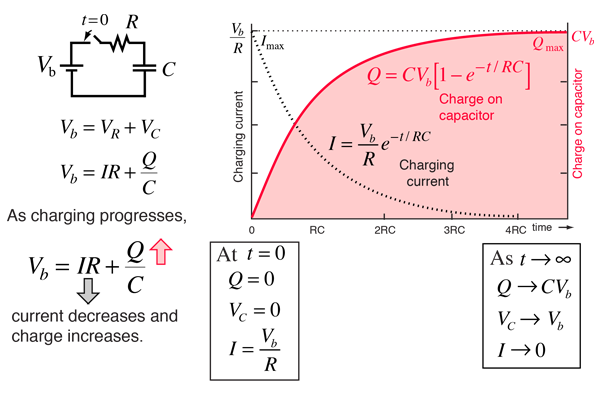
\includegraphics[width=9cm]{curve.png}
		\caption{Capacitor Charging Curve(Source: Hyperphysics)}
		\label{fig:charge}
	\end{figure} \newline \newline
	The time it takes for a capacitor to charge to its 63 percent of its intended amount during charging or to drop to 37 percent of its full amount during discharging is \textbf{RC} seconds. RC is called the time constant and is represented by the Greek letter Tau($\tau$)
	
	\subsection*{Factors Affecting Capacitance}
	A simple parallel plate capacitor contains parallel plates usually with an insulator in between them. The insulator in between the capacitors is called the \textbf{dielectric}. Capacitance can be affected by how much charge the plates can hold and the separation between them. Thus, the area of the plates(\textit{A}) and the separation between them(\textit{d}) are the main factors affecting the capacitance of a parallel plate capacitor.
	
	\begin{equation}
		C = \frac{\varepsilon_0A}{d}
	\end{equation}
	Where:
	\begin{itemize}
		\item $\varepsilon_0$ is a quantity called permitivitty of free space(vacuum) and it is the measure of the tendency of free space to be polarized. 
		\item A is the area of the plates.
		\item d is the separation distance between the plates
	\end{itemize}
	However, we have seen that we usually have an insulator(\textit{dielectric}) between the plates. When that happens, instead of $\varepsilon_0$(Permitivitty of free space), we have $\varepsilon$(Permitivitty of dielctric). Our equation, then, becomes:
	
	$$ C = \frac{\varepsilon A}{d}$$
	Where:
	\begin{itemize}
		\item $\varepsilon$ is the permitivitty of the dielectric.
	\end{itemize}    
	Permitivitty of a dielectric is related to the permitivitty of free space. The ratio between the permitivitty of a dielectric to that of free space is called \textbf{relative permitivitty} or \textbf{dielectric constant} and it is given by the Greek letter kappa($\kappa$).
	$$\kappa = \frac{\varepsilon}{\varepsilon_0}$$	
	\section*{Energy Stored in a capacitor}
	We have discussed previously that the use of capacitors is to store more charge at a lower potential(compared to other electrical equipments such as batteries.) When charges are stored on the plates of a capacitor, there is a potential energy that is stored in the capacitor as the plates are charged and are kept at a distance(think of the plates as point charges and a distance \textbf{r} between them). \\
	To find the energy stored in the capacitor, let's see how a capacitor's charge increases with respect to the voltage. \begin{center}
		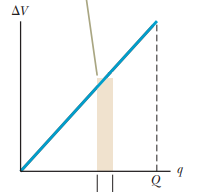
\includegraphics[scale=0.7]{v_q_curve.png}
	\end{center}
	We can see on the graph above that when a capacitor charges, the potential difference increases \textit{proportionally} with the charge being stored. When we have such situations, we take the average value of the charge. Since the charge is increasing with a constant slope, we take the midpoint of the line. \\
	That is,
	$$\frac{Q + 0}{2}$$
	That gives us the average value  of the charge while the potential difference on the plates of the capacitor reach the potential difference of the battery. If we look at the area under the curve of the \textbf{V} vs \textbf{Q} curve, we get the following:
	$$\text{Area}=\frac{1}{2}Q\times V$$
	The area under the line happens to be the energy stored in the capacitor. Thus,
	$$E = \frac{1}{2}Q\times V$$
	We can also express the area in terms of the capacitance and voltage.
	\\
	\newline
	We know that $$Q = C \times V$$
	That means,
	$$E = \frac{1}{2}(C\times V)\times V$$
	$$E = \frac{1}{2}CV^2$$
	
	\section*{Advanced: The meaning of the $\dfrac{1}{2}$}
	To understand the mathematical meaning of the $\frac{1}{2}$ at the beginning of the equation, we can make use of calculus and interested students can look at the following.(Remember how we used calculus to estimate the amount of charge left in a capacitor during discharge?)
	$$dW = \varDelta V\times dq$$
	$$dW = \frac{q}{C}\times dq$$
	To get the work, we integrate both sides:
	$$\int dW =\int_{0}^{Q}\frac{q}{C}dq$$
	$$ W =\frac{q^2}{2C}\Big|_0^Q $$
	$$ W =\frac{q^2}{2C}\Big|_0^Q $$
	$$ W =\frac{Q^2}{2C}$$
	Now, we can see how the $\frac{1}{2}$ has come to presence mathematically.
	\section*{Combination of Resistors}
	More often than not, we will use multiple capacitors in a circuit than just one. Thus, we have to compute the effective capacitance of the circuit.\newline
	We can combine the capacitors through a single path end-to-end with the same charges passing through them. This connection is called a \textbf{series} combination of capacitors. Look at the figure below for an example of a series combination of capacitors. \\
	\begin{center}
		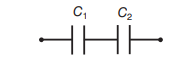
\includegraphics[scale=1]{series_capacitors.png}	
	\end{center}
	In both capacitors, we have the same charges flowing through them. Let the charge provided by the battery be \textbf{Q}, and if these capacitors are connected with series to the battery, a charge of \textbf{Q} passed through each of them. But, the potential difference provided by the battery is divided between the two capacitors. If the potential difference provided by the battery is \textbf{V}, we have the following: \newline
	$$V = V_1 + V_2$$
	We know that $V=\dfrac{Q}{C}$, thus,
	$$\dfrac{Q}{C} = \frac{Q_1}{C_1} + \frac{Q_2}{C_2}$$
	Since all the charges are equal,
	$$Q_1=Q_2=Q$$
	$$\frac{Q}{C} = \frac{Q}{C_1} + \frac{Q}{C_2}$$
	$$\frac{1}{C} = \frac{1}{C_1} + \frac{1}{C_2}$$    
	Thus, the reciprocal of the effective capacitance of the circuit is the reciprocal sum of each capacitance. Here, we can see that the effective capacitance can never be larger than the capacitance of each capacitance.
	In situations where the capacitors are connected in parallel(when the wire \textbf{branches} out), as in the figure below,\\
	\begin{center}
		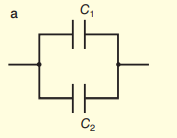
\includegraphics[scale=1]{parallel_capacitors.png}	
	\end{center}
	We have the potential difference to be the same for the capacitors connected in parallel. However, the charge from the battery is the sum of the charge in each capacitor.
	$$V = V_1 = V_2$$
	But we know that:
	$$Q=CV$$
	And,
		$$Q = Q_1 + Q_2$$
	$$CV= C_1V_1 + C_2V_2$$
	$$CV = V(C_1+C_2)$$
	$$C = C_1 + C_2$$
	This means that the effective capacitance of capacitors connected in parallel. is the sum of each capacitance.
		\begin{center}
		\section*{Homework 5}
		\subsubsection*{Information}
		\begin{itemize}
			\item The homework is due on \textbf{Friday}, \textbf{December 30th}.
			\item You should Work on it \textbf{individually} and consult me if you have any questions. As I have reiterated multiple times, cheating will have a serious consequence.
			\item For purposes of neatness and simplicity of grading, you should do the homework on an \textbf{A-4 paper}.
		\end{itemize}
	\end{center}
	\begin{center}
		\subsection*{Questions}
	\end{center}
	
	\begin{questions}
		\question Define electric potential and describe its relationship with electric potential energy.
		\question When a 1.5 V flashlight battery runs a single 20W headlight, how many electrons pass through it each second?
		\question What is the difference between a car battery that is 12V and a smaller flashlight that is also 12V? Why does the latter run out faster although they have the same voltage?
		\question A lot of electrical appliances have potential differences set at some reference point. As you may recall, potential difference is the difference in absolute potential between points. For example, a voltaic cell might have a voltage of 1.5V, what does that mean? Also, why do we have ground as a reference in multiple electric appliances?
		\question How far apart are two conducting plates that have an electric field strength of  6.40×$10^3$V/m  between them, if their potential difference is 8.0kV?		
		\subsection*{Challenge Problems}
		\textit{\textbf{The following challenge problems are not required to be submitted, but are highly encouraged}.} \\
		\question Find the ratio of speeds of an electron and a negative hydrogen ion (one having an extra electron) accelerated through the same voltage.
		\question Why are equipotential lines and surfaces perpendicular to the electric field lines?
		\question A lightning bolt strikes a tree, moving 30.0 C of charge through a potential difference of 1.00×10$^2$MV.\begin{itemize}
			\item What energy was dissipated?
			\item  What mass of water could be raised from  room temperature(25$^0$c) to the boiling point and then boiled by this energy?
			\item Discuss the damage that could be caused to the tree by the expansion of the boiling steam.
		\end{itemize} 
	\end{questions}		
		\begin{center}
		\subsection*{Group Work Requirements}
	\end{center}
	\subsubsection*{Original Content \& No direct plagiarism } 
	The paper you submit should be as original as possible and not a direct plagiarized content from others' work. To that end, the originality of your paper has a weight of \textbf{25}\%.
	\subsubsection*{Actuality \& Scientific Truth}
	The paper submitted should be based on a scientifically accepted truth/fact. This, again, has a weight of \textbf{25}\%.
	\subsubsection*{Written in Proper English}
	The paper submitted should be written in a language that is grammatically correct and should make sense. This has a weight of \textbf{20}\%
	\subsubsection*{Presentation \& Slides}
	The group project will be presented and should have PowerPoint /Beamer slides. The presentation along with the quality of the slides has a weight of \textbf{30}\% \\ \\
	\textbf{Extrapoints}\\
	As an incentive to push all of you into scientific endeavors, there will be extra points for doing the following:
	\begin{itemize}
		\item A paper written in LaTex.
		\item Slides made with Beamer.
		\item If you include relevant material in your presentation or provide in addition(for instance, could be codes for simulations)
	\end{itemize}
	The maximum extra points you will get will be 20\% of the total weight of the project.
	
	\end{document}	